% !TeX root=../main.tex
\chapter{دست‌آوردها، پیشنهاد‌ها، محدودیت‌ها}

\section{دست‌آوردها}

\subsection{پلتفرم ایجاد شده}
قرارداد هوشمند نوشته شده در این پروژه،
کاپو، با عملکرد کامل بر بروی شبکه تستی راپستن بارگذاری شد
و امکانات لازم برای دسترسی عموم مردم به روشی آسان و ارزان به توکن‌های تعویض ناپذیر را فراهم می‌کند.
کاربران می‌توانند در صفحه اصلی این اپلکیشن تعداد توکن‌های ساخته شده و تعداد آدرس‌های دارای توکن را مشاهده کنند.
سپس با متصل کردن کیف‌پولشان به اپلیکیشن می‌توانند توکن بسازند،
دارایی‌هایشان را مشاهده کنند و توکن‌هایشان رو به دیگران ارسال کنند.

\subsection{ساخت محیط توسعه سریع و خودکار}
سپس آموختیم که چگونه اجرای تست‌های قرارداد هوشمند را داکرایز و به صورت خودکار در پایپ‌لاین پروژه اجرا کنیم.
برای انجام این کار یک داکر ایمیج ترافل نوشته شد،
کد آن به صورت متن‌باز بر روی گیت‌هاب بارگزاری و ایمیج آن به داکرهاب اضافه شد. سپس واسط کاربری اپلیکیشن داکرایز شد و از
\lr{env}
های داکر برای فرستادن توکن گیت‌هاب از پایپلاین به کانتینر استفاده شد
و در نتیجه واسط کاربری اپلیکیشن به صورت خودکار در پایپلاین پروژه روی صفحات گیت‌هاب بارگزاری می شود.

در نتیجه انجام این کارها یک مسیر راحت و سریع برای توسعه یک قرارداد هوشمند به همراه واسط کاربری ایجاد شد که تست‌ها
و فرایند بارگذاری همه به صورت خودکار در آن اجرا می‌شوند.


\subsection{ورود به
\gls{Community}}
برای انجام این پروژه از قرارداد‌های هوشمند اپن‌زپلین استفاده شد.
اپن‌زپلین یکی از پر استفاده‌ترین مخزن استانداردهای قراردادهای هوشمند است
که در زمان نوشته شدن این متن در گیت‌هاب بیش از هفده هزار و پانصد ستاره و نزدیک به نه هزار فورک دارد.
در حین توسعه کاپو تغییراتی در پروژه اپن‌زپلین نیز اعمال گردید.
سپس یک
\gls{Merge Request}
شامل این تغییرات ساخته شد که در همان روز توسط تیم اپن‌زپلین به مخزن کد اصلی اضافه شد.
این مرج ریکوئست در تصویر
\ref{fig:oz-mergereq}
قابل مشاهده است.
این موضوع برتری‌های توسعه متن‌باز را نشان می‌دهد.
تیم‌های توسعه بزرگ، حتی به بزرگی پروژه‌ای مانند اپن‌زپلین، از کمک همه توسعه دهندگان استقبال می‌کنند،
حتی کسانی که برای اولین بار می‌خواهند روی یک پروژه تغییری ایجاد کنند.


\begin{figure}[H]
\centerline{\frame{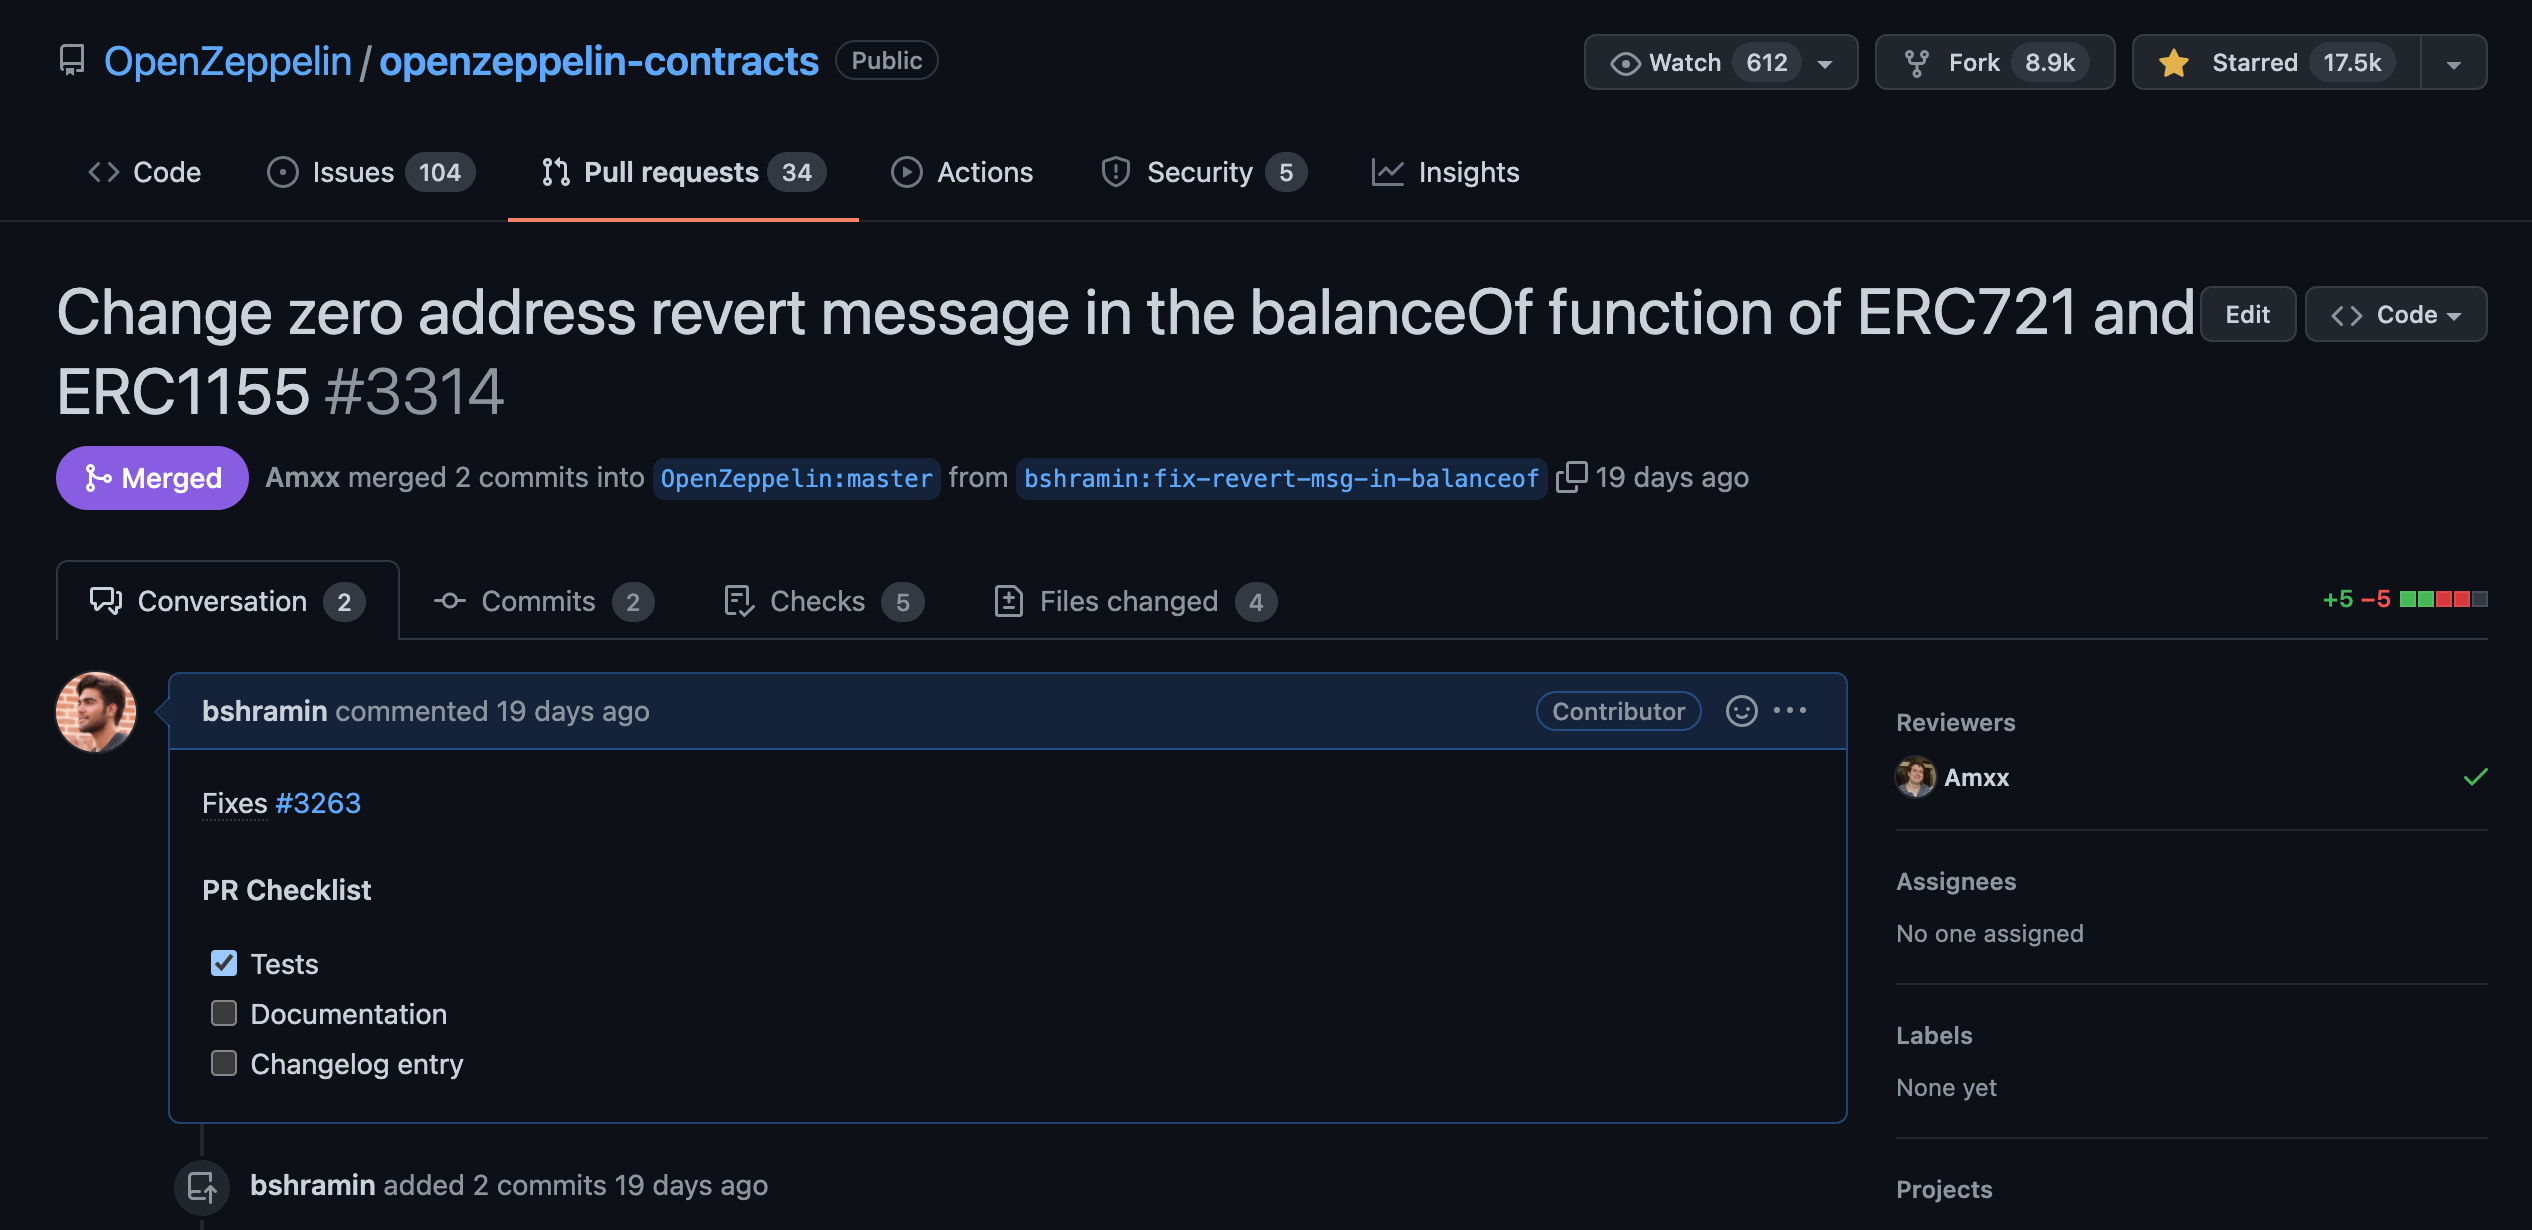
\includegraphics[width=12cm]{oz-mergereq.png}}}
\caption{مرج ریکوئست باز شده بر روی اپن‌زپلین}
\label{fig:oz-mergereq}
\end{figure}


\subsection{یادگیری}
در طی انجام این پروژه با ابزارها، چارچوب‌ها، کتابخانه‌ها و استانداردهای توسعه قراردادهای هوشمند آشنا شدیم.
آموختیم که چارچوب ترافل چه ابزارهایی را در اختیار توسعه دهنده قرار می‌دهد.
چگونه می‌توان یک شبکه محلی برای توسعه ایجاد کرد،
قرارداد هوشمند را بر روی آن بارگذاری کرد و واسط کاربری و کیف پول را به آن متصل کرد.

آموختیم که چگونه می‌توانیم برای پیاده‌سازی قراردادهای هوشمند از استانداردهای موجود استفاده کنیم،
برای آن‌ها تست بنویسیم و به کمک چارچوب ترافل این تست‌ها را اجرا کنیم.
آموختیم که چگونه پس از اتمام فرآیند توسعه قرارداد هوشمند را بر روی شبکه تستی بارگذاری کنیم.
همچنین واسط کاربری اپلیکیشن به کمک صفحات گیت‌هاب بارگذاری و به قرارداد هوشمند روی شبکه تست متصل شد.


\section{پیشنهادها}
در این قسمت با توجه به آموخته‌هایی که در طی انجام این پروژه به دست آمد،
پیشنهادهایی برای توسعه پروژه‌های مشابه ذکر می شود.
امید است که استفاده از این پیشنهادها مسیر توسعه را هموارتر کرده و سرعت ببخشد.

\subsection{استفاده از استانداردها}
خوشبختانه در این پروژه از ابتدا به استفاده از استانداردهای موجود اهمیت داده شد.
در صورتی که توسعه دهنده بخواهد از استانداردهای موجود استفاده نکند مزیت سازگاری
قرارداد هوشمند نوشته شده با پلتفرم‌هایی که از پیش وجود دارند را از دست می‌دهد.

همچنین در صورتی که توسعه دهنده تصمیم بگیرد که از یکی از استانداردها پیروی کند
بهتر است که از پیاده‌سازی‌های موجود به صورت متن‌باز استفاده کند، این تصمیم باعث
رشد چشمگیر سرعت توسعه قرارداد هوشمند می‌شود، امکان وجود خطا و مشکل امنیتی در قرارداد را کم
و امکان دریافت آپدیت‌های جدید را تسهیل می‌کند.


\subsection{استفاده از \lr{ERC1155} به جای \lr{ERC721}}
استاندارد
\lr{ERC1155}
برتری‌های فراوانی نسبت به استاندارد
\lr{ERC721}
دارد.
از جمله این برتری‌ها می‌توان به قابلیت ارسال چند توکن در یک تراکنش،
توانایی ساخت انواع مختلف توکن با تعداد متفاوت و
پشتیبانی از توکن‌های تعویض‌پذیر و تعویض‌ناپذیر به صورت همزمان اشاره کرد.
با توجه به قابلیت ارسال هم‌زمان چند توکن و یا ساخت هم‌زمان چندین توکن در یک تراکنش،
هزینه‌ی پرداختی کاربرها نیز
برای استفاده از قرارداد هوشمند به نحو شایانی کاهش می‌یابد و به این نحو قرارداد در دسترس
جامعه بزرگتری قرار می‌گیرد.

\subsection{ساخت محیط توسعه از شروع کار}
انجام مواردی مانند خودکار سازی اجرا شدن تست‌ها،
بارگذاری رابط کاربری و استفاده از ابزارهای کنترل ورژن مانند گیت‌هاب
گرچه در شروع کار ممکن است خسته‌کننده باشند و به توسعه‌دهنده حس پیشرفت در انجام پروژه را ندهند، اما
این کارها هرچه زودتر و در شروع پروژه انجام شوند سرعت پیشرفت پروژه را دو چندان می‌کنند.
در نتیجه پیشنهاد می‌شود که در نقطه شروع پروژه به روند توسعه توجه شود و زمانی به
بهینه‌سازی این روند اختصاص داده شود.


\section{محدودیت‌ها}

\subsection{استفاده از
\gls{Drizzle}
}
در ابتدای انجام پروژه سعی شد که برای برقراری ارتباط رابط کاربری با قرارداد هوشمند از دریزل استفاده شود.
اما استفاده از این ابزار مشکلات فراوانی را به همراه داشت.
با توجه به تازگی و بالغ نبودن ابزارهای موجود برای توسعه قراردادهای هوشمند،
باید سعی شود که تا جای ممکن از ابزارهای پراستفاده و با
\gls{Community}
بزرگ استفاده شود. در این پروژه پس از مواجهه با محدودیت‌های فراوان دریزل،
از کتابخانه‌ \lr{Web3JS} استفاده شد که دست توسعه دهنده را به میزان خوبی باز می‌گذارد.

\subsection{ورژن‌های مختلف ابزارها}
عدم همخوانی نسخه‌های مختلف ابزارهای مورد استفاده با یکدیگر مشکلات زیادی در توسعه پروژه ایجاد کرد.
در هنگام توسعه پروژه باید حتما دقت شود که برای هر ابزار در حال استفاده از چه نسخه‌ای هستیم.
همچنین برای محدود کردن این مشکل پیشنهاد می‌شود از ابزارهای کانتینر کننده مانند داکر استفاده شود.

\subsection{هزینه تراکنش‌های شبکه اصلی اتریوم}
در زمان نوشته شدن این متن، هزینه انجام تراکنش روی شبکه اصلی اتریوم به شدت بالاست.
این هزینه‌ی بالا باعث می‌شود که بارگذاری کردن روی شبکه اصلی برای یک پروژه آزمایش از دسترس دور باشد.
اگرچه ممکن است در آینده با بروزرسانی اتریوم ۲ این هزینه به شدت کاهش یابد.

\subsection{عدم وجود راهنما و مستندات کافی}
تازگی این زمینه باعث عدم وجود راهنما و مستندات کافی شده است.
این موضوع از دیگر دلایل پیشنهاد به استفاده از ابزارهای با جامعه توسعه‌دهندگان بزرگ است.
